%Corps du document :
%\setlength{\parindent}{1cm}    

\section{Conception détaillée des applications}

\subsection{Diagramme d'enchaînement des fenêtres}

\begin {center}
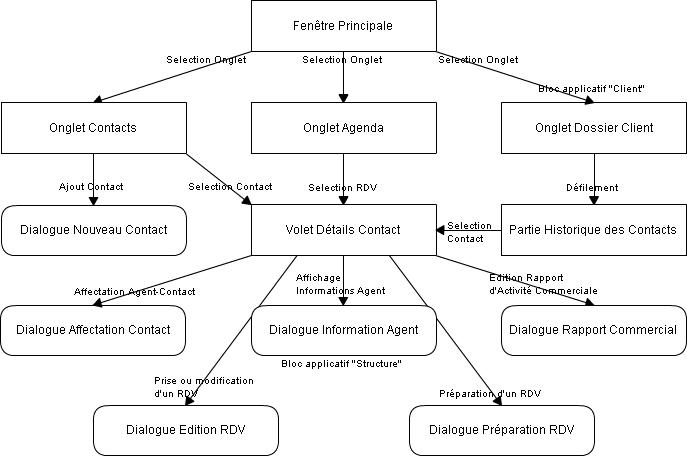
\includegraphics[width=\textwidth]{diagramme-edf.png}
\end {center}

La fenêtre principale présente trois onglets principaux :

\begin{itemize}
\item La Liste des Contacts : Si l'utilisateur est le chef d'agence, elle montre tous les contacts prévus et permet de les affecter à des agents, sinon elle montre simplement les contacts affectés à un agent et permet de prendre Rendez-Vous avec le client. Suite à la demande d'un client, un agent peut également ajouter un contact manuellement.
\item L'Agenda : Il permet de situer les Rendez-Vous dans le temps grâce à une vue calendaire paramétrable. Un Rendez-Vous peut être modifié, préparé, et une fois qu'il a été effectué, l'interface permet de rédiger un Rapport d'Activité Commerciale pour cloturer le contact.
\item Dossier Client : TODO
\end{itemize}